\chapter{Appendix C --- Supplementary Figures}
\label{ch:appendixC}

This appendix contains the graphical results of some experiments made througout
this work which were glossed over in the main text, but shall be provided here
for completeness and the reader's enjoyment.

\section*{\texttt{ikkuna} for Optimiser Research}%
\label{sec:ikkuna_for_optimiser_research}

In \cref{subsec:adam-behaviour} we plotted exponential moving averages of
gradients and squared gradients, as well as the effective per-layer learning
rate Adam would use. In this section we provide the remaining parameter
combinations of this experiment.

\begin{figure}
    \begin{subfigure}{\textwidth}
        \centering
        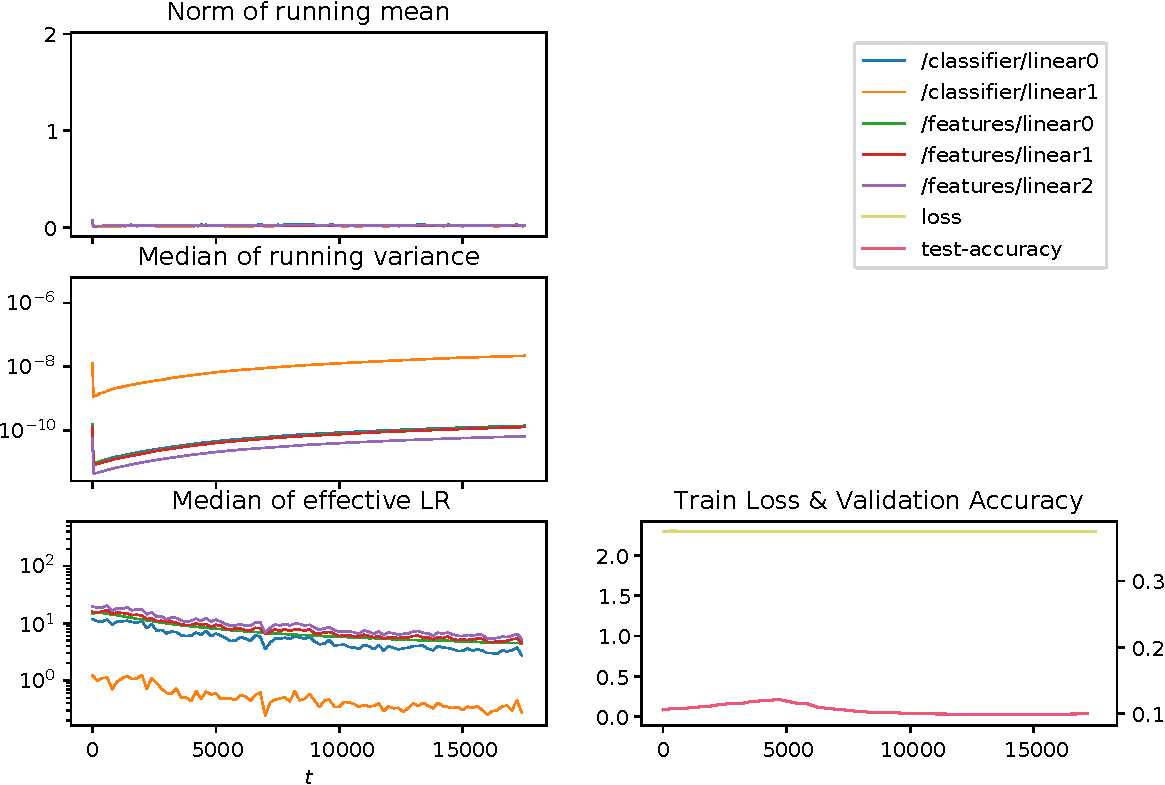
\includegraphics[width=\linewidth]{gfx/diagrams/experiments/adam/fullyconnectedmodel_sgd_00005_0_-1.pdf}
        \caption{Dense model with learning rate $0.0005$, optimised with SGD}
    \end{subfigure}

    \begin{subfigure}{\textwidth}
        \centering
        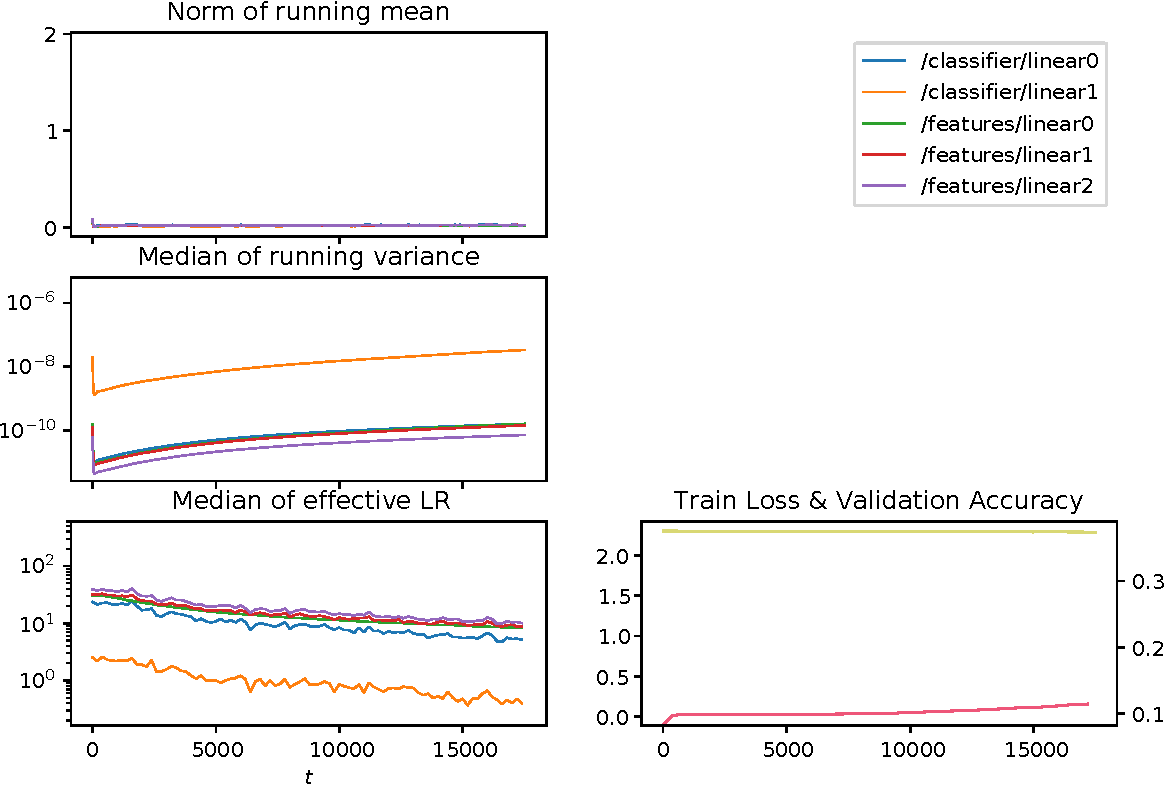
\includegraphics[width=\linewidth]{gfx/diagrams/experiments/adam/fullyconnectedmodel_sgd_0001_0_-1.pdf}
        \caption{Dense model with learning rate $0.001$, optimised with SGD}
    \end{subfigure}

    \begin{subfigure}{\textwidth}
        \centering
        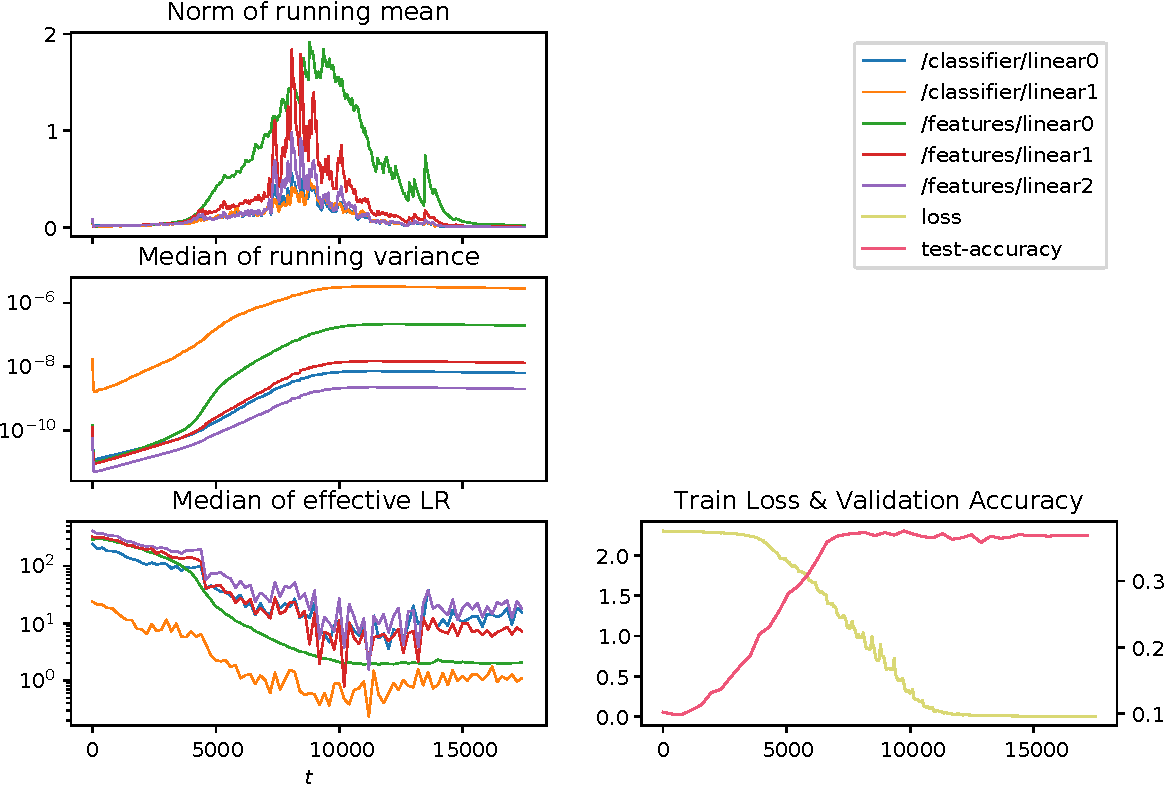
\includegraphics[width=\linewidth]{gfx/diagrams/experiments/adam/fullyconnectedmodel_sgd_001_0_-1.pdf}
        \caption{Dense model with learning rate $0.01$, optimised with SGD}
    \end{subfigure}
    \caption{Adam moments on a purely dense model trained with SGD}
\end{figure}

\begin{figure}
    \begin{subfigure}{\textwidth}
        \centering
        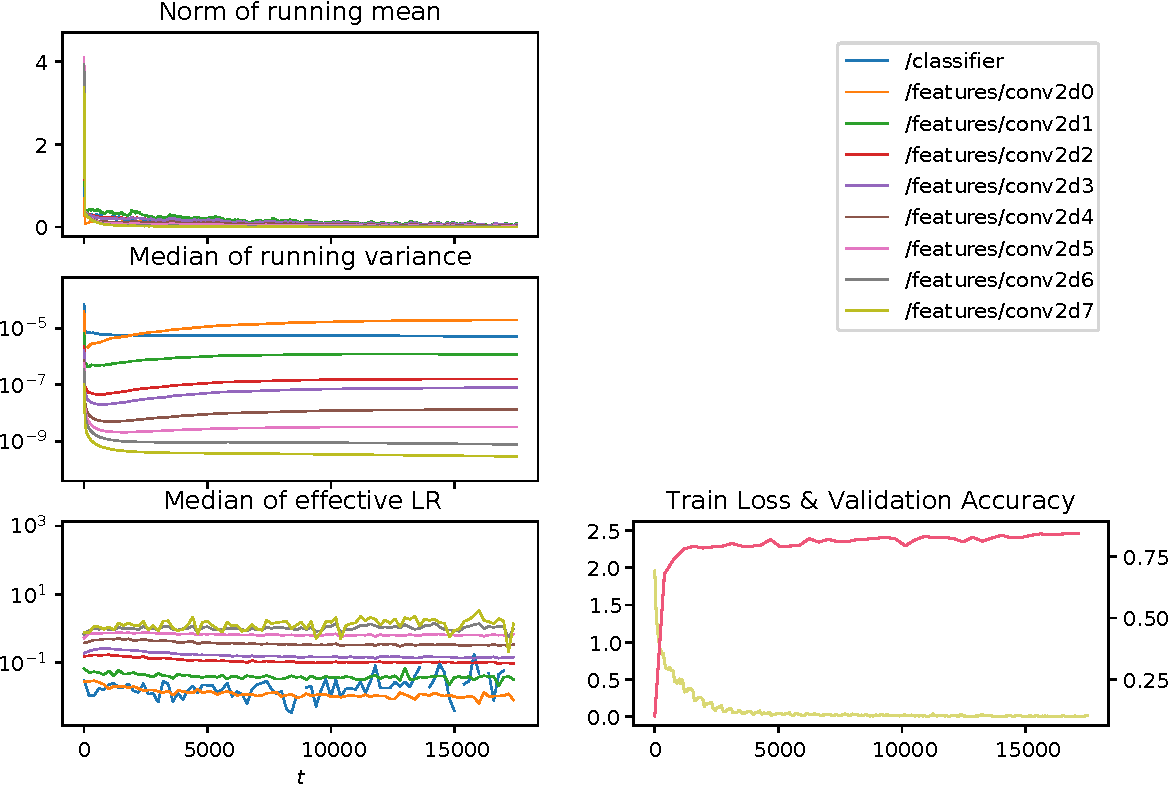
\includegraphics[width=\linewidth]{gfx/diagrams/experiments/adam/vgg_adam_00005_0_-1.pdf}
        \caption{VGG with learning rate $0.0005$, optimised with Adam}
    \end{subfigure}

    \begin{subfigure}{\textwidth}
        \centering
        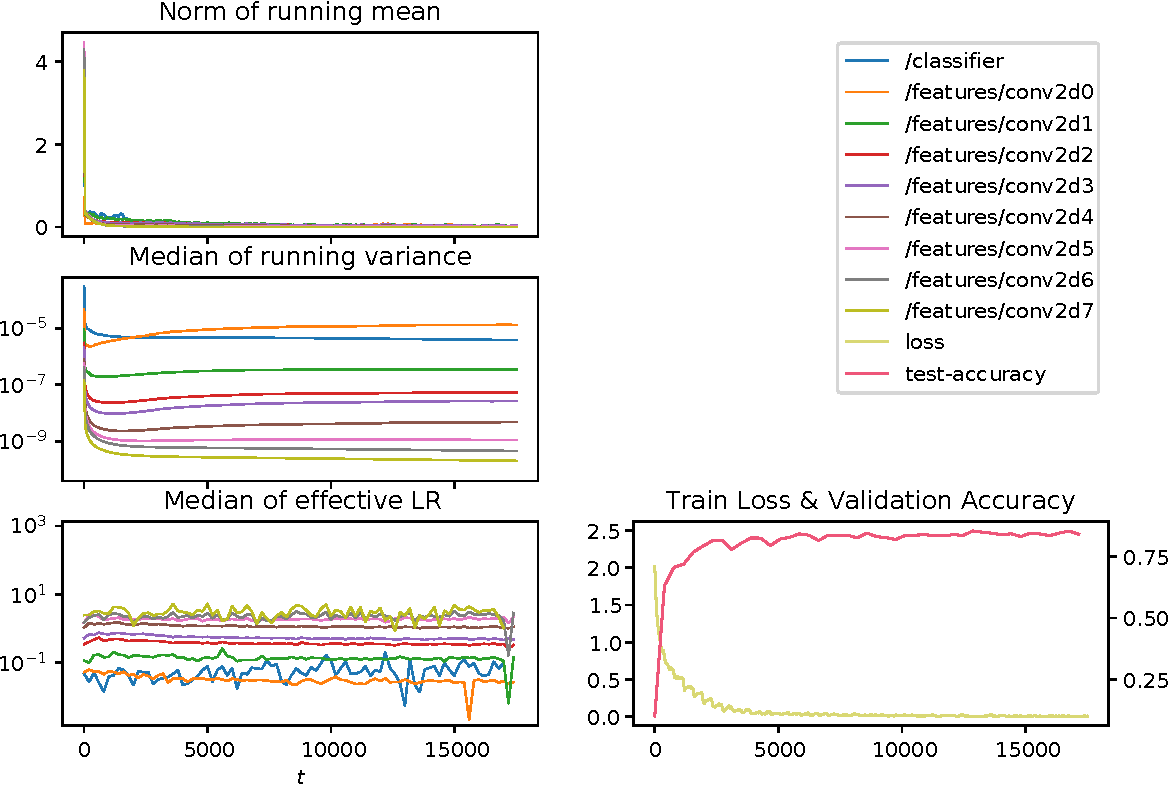
\includegraphics[width=\linewidth]{gfx/diagrams/experiments/adam/vgg_adam_0001_0_-1.pdf}
        \caption{VGG with learning rate $0.001$, optimised with Adam}
    \end{subfigure}

    \begin{subfigure}{\textwidth}
        \centering
        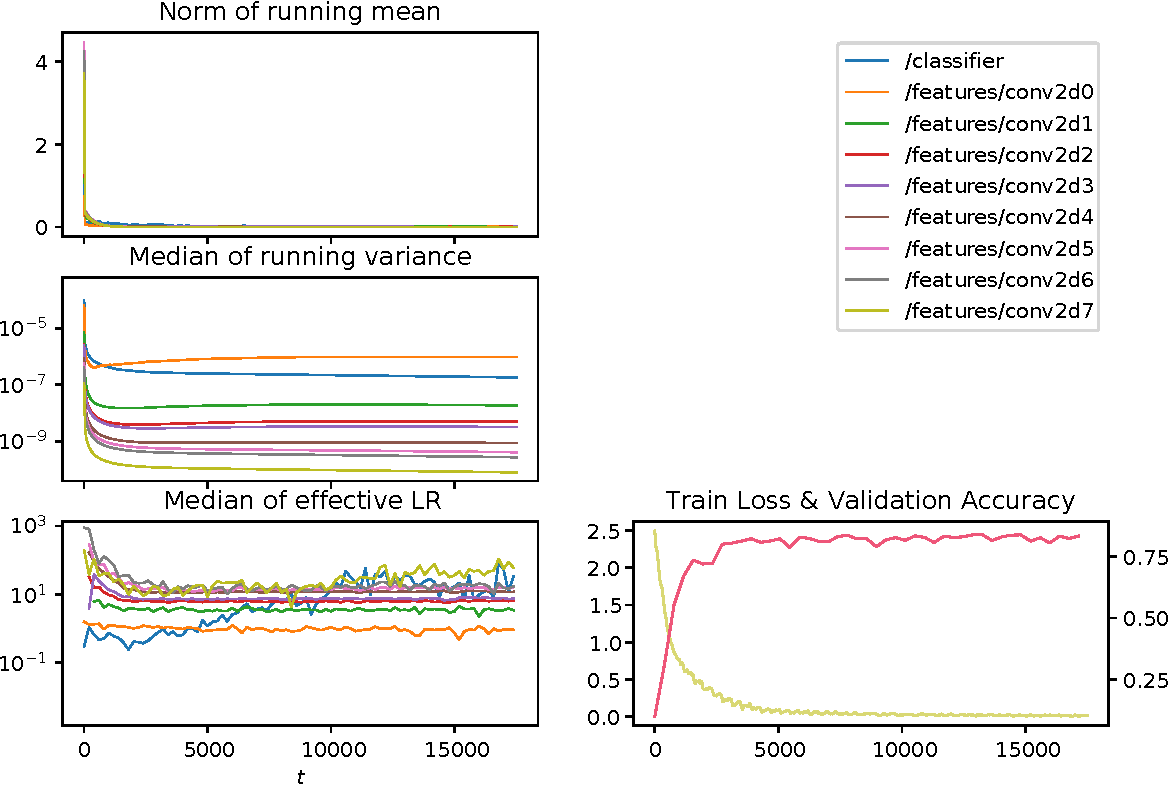
\includegraphics[width=\linewidth]{gfx/diagrams/experiments/adam/vgg_adam_001_0_-1.pdf}
        \caption{VGG with learning rate $0.01$, optimised with Adam}
    \end{subfigure}
    \label{fig:vgg-experiment}
    \caption{Adam moments on a VGG model trained with Adam}
\end{figure}

\begin{figure}
    \begin{subfigure}{\textwidth}
        \centering
        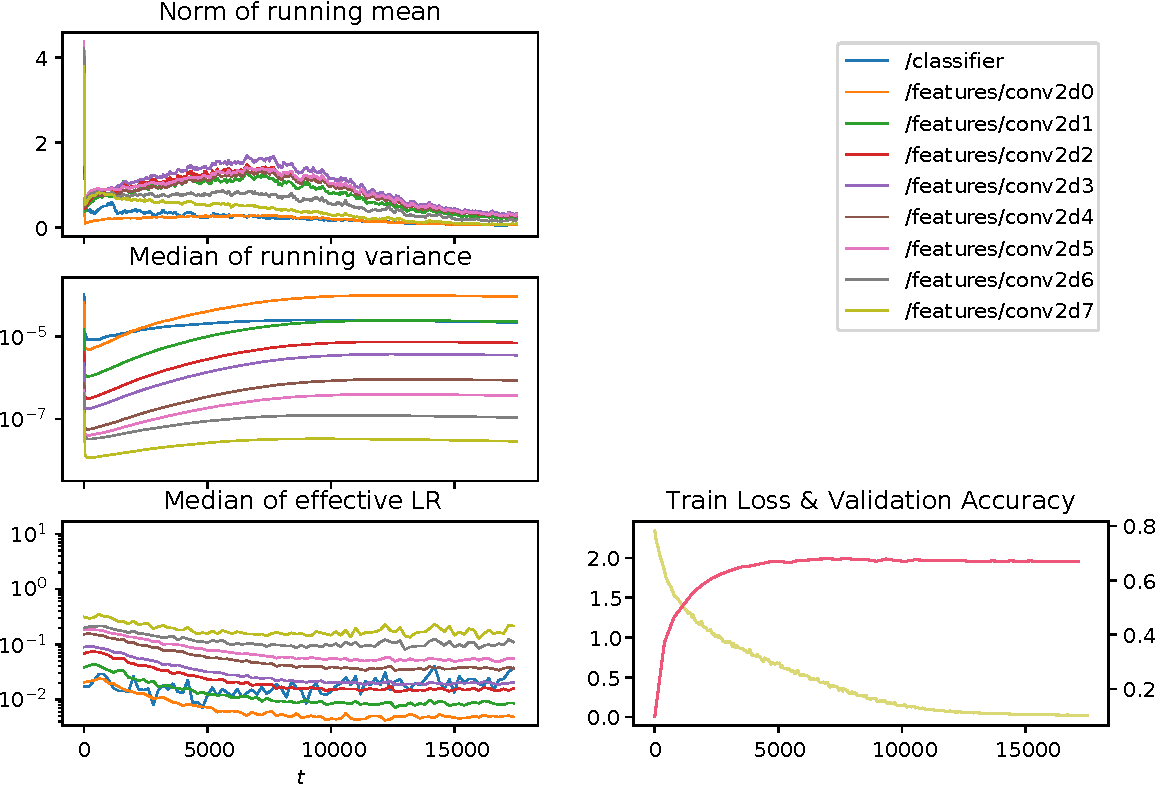
\includegraphics[width=\linewidth]{gfx/diagrams/experiments/adam/vgg_sgd_00005_0_-1.pdf}
        \caption{VGG with learning rate $0.0005$, optimised with SGD}
    \end{subfigure}

    \begin{subfigure}{\textwidth}
        \centering
        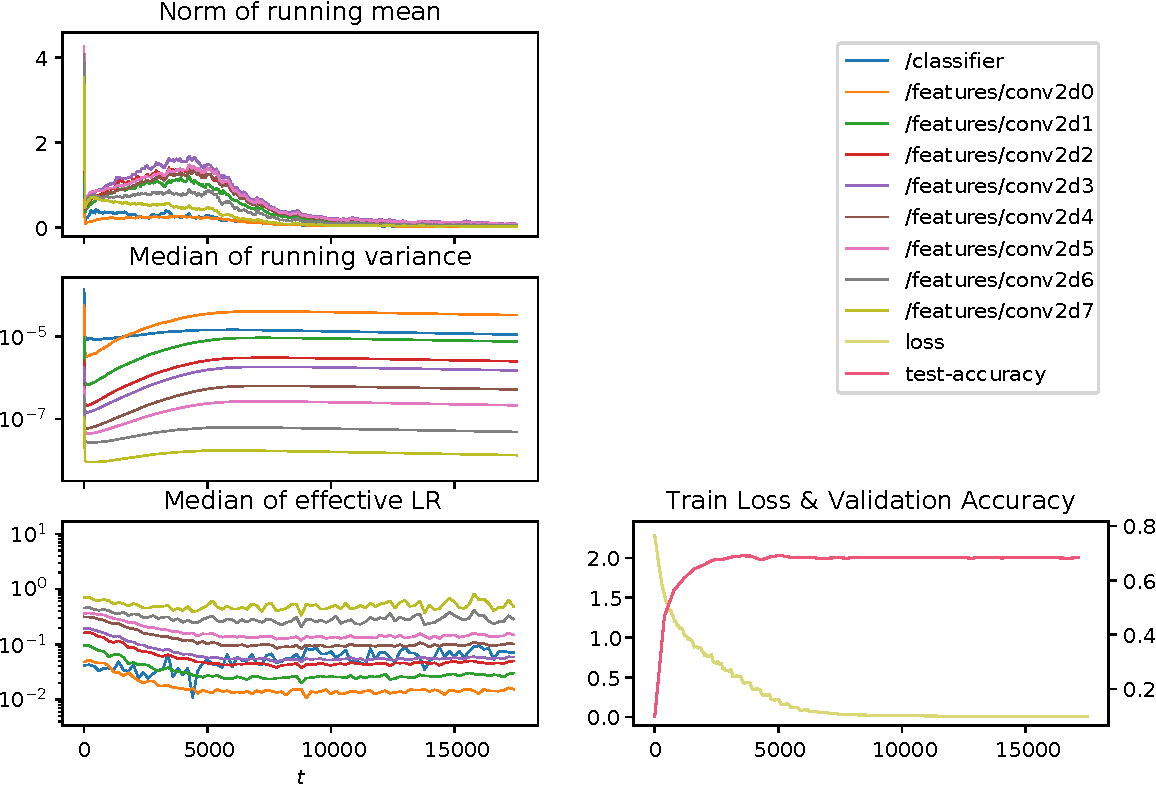
\includegraphics[width=\linewidth]{gfx/diagrams/experiments/adam/vgg_sgd_0001_0_-1.pdf}
        \caption{VGG with learning rate $0.001$, optimised with SGD}
    \end{subfigure}

    \begin{subfigure}{\textwidth}
        \centering
        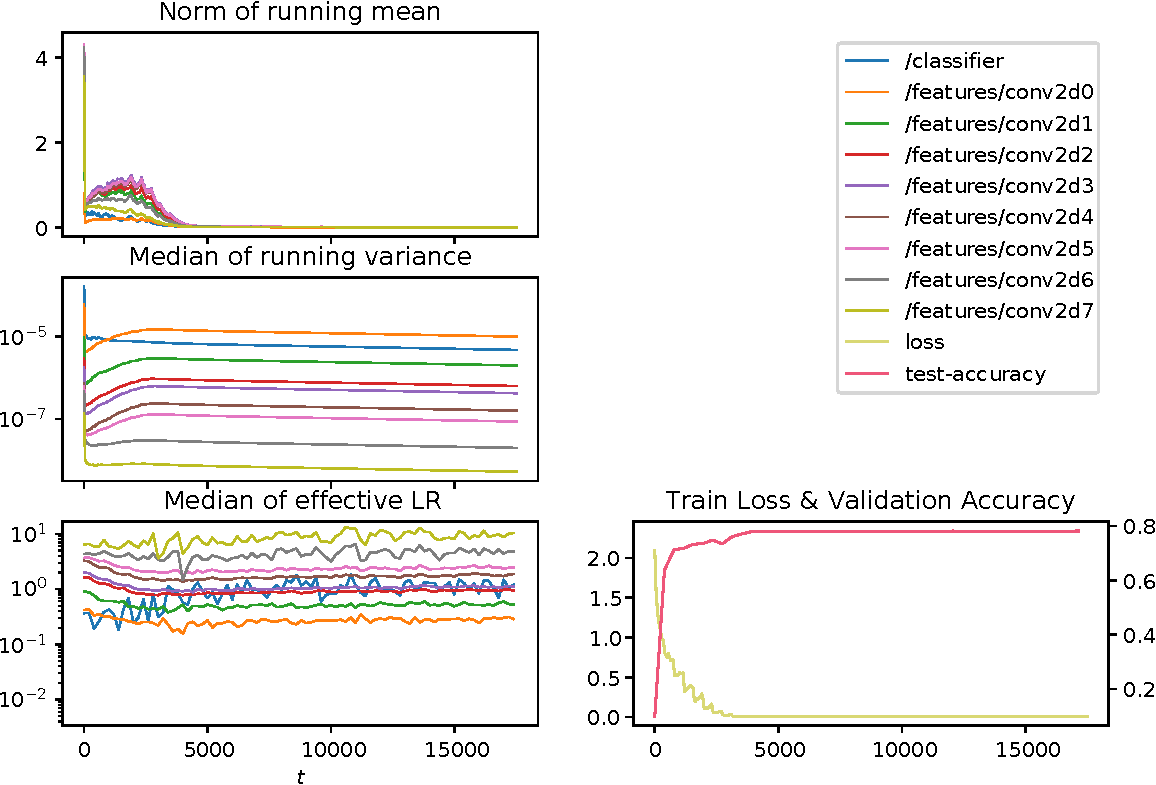
\includegraphics[width=\linewidth]{gfx/diagrams/experiments/adam/vgg_sgd_001_0_-1.pdf}
        \caption{VGG with learning rate $0.01$, optimised with SGD}
    \end{subfigure}
    \label{fig:vgg-experiment-sgd}
    \caption{Adam moments on a VGG model trained with SGD}
\end{figure}
